\chapter{Resultados}

Além da análise da facilidade de uso e implementação paralela desses algoritmos, para analisar o custo-benefício real das duas implementações é preciso primeiramente verificar se os resultados obtidos são corretos, e posteriormente o quão grande foi a redução do tempo de execução comparado a versão sequencial dos algoritmos. Nesse capítulo será estudado esses dois fatores.

\section{Autenticação dos resultados}

Algo imprescindível em algoritmos de processamento e análise de dados para que possam ser efetivamente usados em pesquisas é a confiabilidade dos resultados obtidos. Nem sempre é possível apenas observando os resultados saber se o mesmo esta certo ou errado. Portanto é preciso ter total confiança de que os dados obtidos da execução do algoritmo estão corretos.

Por esse motivo, o pequeno número de alterações feitas no código é tão importante, pois evita que erros sejam cometidos no processo de conversão. Além disso, em todos os testes realizados, os resultados obtidos da versão CUDA foram comparados com os do sequencial, e em todos os casos os mesmos foram idênticos, comprovando que os resultados estão corretos.

\section{Avaliação do tempo de execução}

Contudo, a principal motivação da implementação paralela desses algoritmos é a redução do tempo de execução e se tal melhora faz valer todo o esforço. Para comparar o desempenho das implementações em OpenMP e CUDA com a implementação sequencial foram realizados diversos testes, com diferentes parâmetros, e em diferentes configurações de Hardware, com o intuito de medir o tempo real de execução dos mesmos para então verificar se houve uma redução significativa desse tempo.

Nos testes da implementação em OpenMP foram utilizados os seguintes processadores:

\begin{itemize}
\item AMD Opteron
\item Intel I5
\item Intel I7
\end{itemize}

Já nos testes da implementação em CUDA foram utilizados as seguintes placas-de-vídeo:

\begin{itemize}
\item NVidia	 9600GT - 512MB / 900MHz
\item NVidia GTX480 - 1.5GB / 1.4GHz
\end{itemize}

Além disso, na versão CUDA foi utilizado como parâmetro de execução 64 threads por bloco. O número total de blocos e ciclos foram calculados diretamente pelo programa em relação ao tamanho do dado de entrada. Sendo assim, é perceptível que não foi feita nenhuma calibração mais otimizada. Tal decisão foi feita propositalmente em vista que tais ajustes podem variar de uma máquina para outra ou até mesmo de uma entrada para outra, e assumindo que tais programas deverão ser executados por pesquisadores e que os mesmos não teriam tempo e/ou conhecimento para fazer tais ajustes.

Os tempos foram marcados utilizando o comando \texttt{time} do Linux, e portanto são referentes a execução completa do programa, e não só apenas da execução do algoritmo de processamento em si.

\subsection{Resultados obtidos com o algoritmo Filtro de Lanczos}

lala

%%%%%%%%%%%%%%%%%%%%%%%%%%%%%%%%%%%%%%%%%%%%%%%%%%%%%%%%%%
% FIGURA
\begin{figure}[H]
\centering
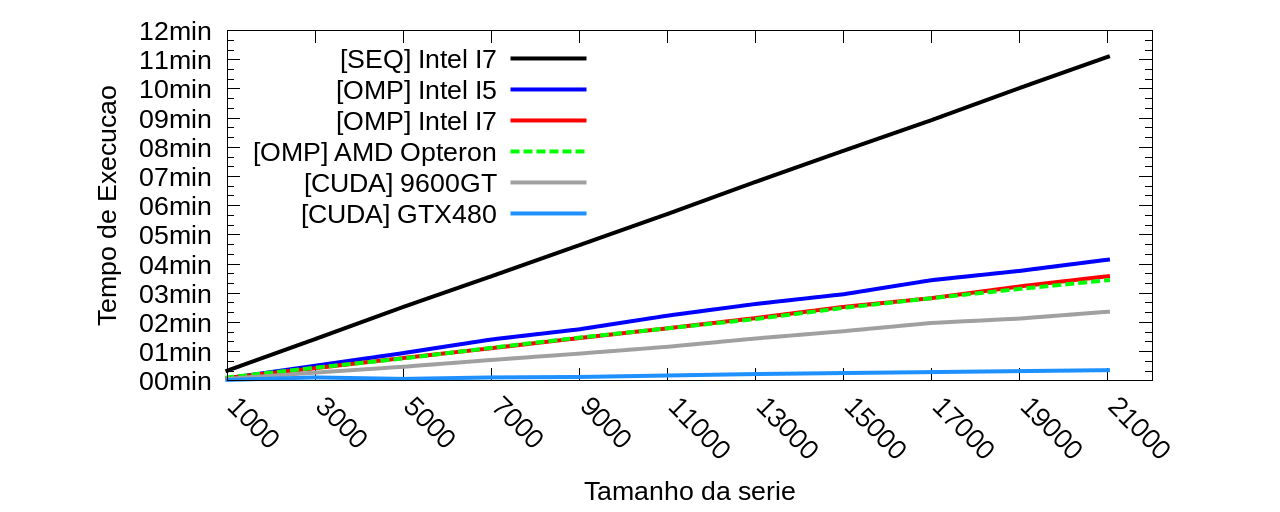
\includegraphics[width=1.0\textwidth]{Imagens/graficos_lanczos/lanczos_tempos.png}
\caption{Gráfico de tempo do algoritmo Filtro de Lanczos}
\label{fig:grafico_tempo_lanczos}
\end{figure}
%%%%%%%%%%%%%%%%%%%%%%%%%%%%%%%%%%%%%%%%%%%%%%%%%%%%%%%%%%

%%%%%%%%%%%%%%%%%%%%%%%%%%%%%%%%%%%%%%%%%%%%%%%%%%%%%%%%%%
% FIGURA
\begin{figure}[H]
\centering
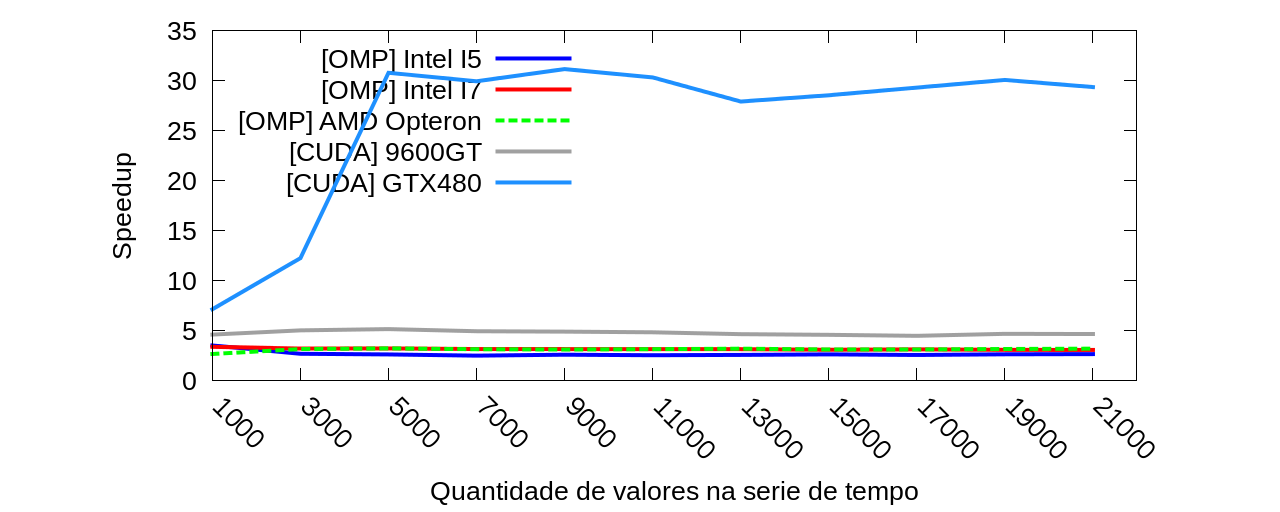
\includegraphics[width=1.0\textwidth]{Imagens/graficos_lanczos/lanczos_speedup.png}
\caption{Gráfico do speedup do algoritmo Filtro de Lanczos}
\label{fig:grafico_speedup_lanczos}
\end{figure}
%%%%%%%%%%%%%%%%%%%%%%%%%%%%%%%%%%%%%%%%%%%%%%%%%%%%%%%%%%

\subsection{Resultados obtidos com o algoritmo Teste de Monte Carlo}

Nos testes do algoritmo de Monte Carlo foram usados como dados de entrada uma matriz de 48 por 56 que contém as informações da quantidade de chuva diária na América do Sul entre os anos de 1979 e 1999, totalizando 7665 valores por série, e uma série de chuvas de um local na África do mesmo comprimento.
Porém, para questão de comparação, o total de valores usados nos testes foi variado entre 1000 e 5000. Da mesma forma o número de permutações foi variado entre 1000 e 9000.

Nos testes da implementação em OpenMP houve uma grande surpresa, pois o tempo de execução foi incrementado em relação ao tempo de execução sequencial, especialmente ao elevar o número de permutações, como pode ser visto na figura \ref{fig:grafico_tempo_mcarlo_omp}. No entanto, nos testes da implementação em CUDA houve uma drástica redução desse tempo, inclusive ao incrementar o número de permutações, como mostrado na figura \ref{fig:grafico_tempo_mcarlo_cuda}.

Uma teoria que explique tais resultados é que pelo fato da implementação em OpenMP prover de apenas uma memória que é compartilhada entre todas as threads, ao se fazer as permutações das séries são realizadas inúmeras requisições simultâneas de escrita na memória que por sua vez não é capaz de responder todas elas imediatamente. Esse atraso faz com que as threads fiquem ociosas durante um longo tempo até que todas as requisições sejam executadas. Ao aumentar o número de permutações o número de requisições é proporcionalmente incrementado agravando o problema.

Tal problema não ocorre na implementação em CUDA pois a mesma é executada na GPU, que possui uma arquitetura de memória totalmente diferente a qual provêm a cada bloco de threads uma memória própria. Dessa forma as requisições de escrita são distribuídas entre várias memórias independentes reduzindo o congestionamento de requisições.

Para reforçar essa hipótese foi feito alguns testes reduzindo o número de threads usadas na execução da implementação em OpenMP. Esses resultados estão expostos na figura \ref{fig:grafico_speedup_mcarlo_omp_threads}. É perceptível que ao reduzir o número de threads o tempo de execução reduz consideravelmente, pois o total de requisições simultâneas também é reduzida e assim amenizando o problema.

Esses resultados são importantes para demonstrar que a arquitetura atual dos computadores não é a ideal para se executar algoritmos paralelos.

%%%%%%%%%%%%%%%%%%%%%%%%%%%%%%%%%%%%%%%%%%%%%%%%%%%%%%%%%%
% FIGURA
\begin{figure}[H]
\centering
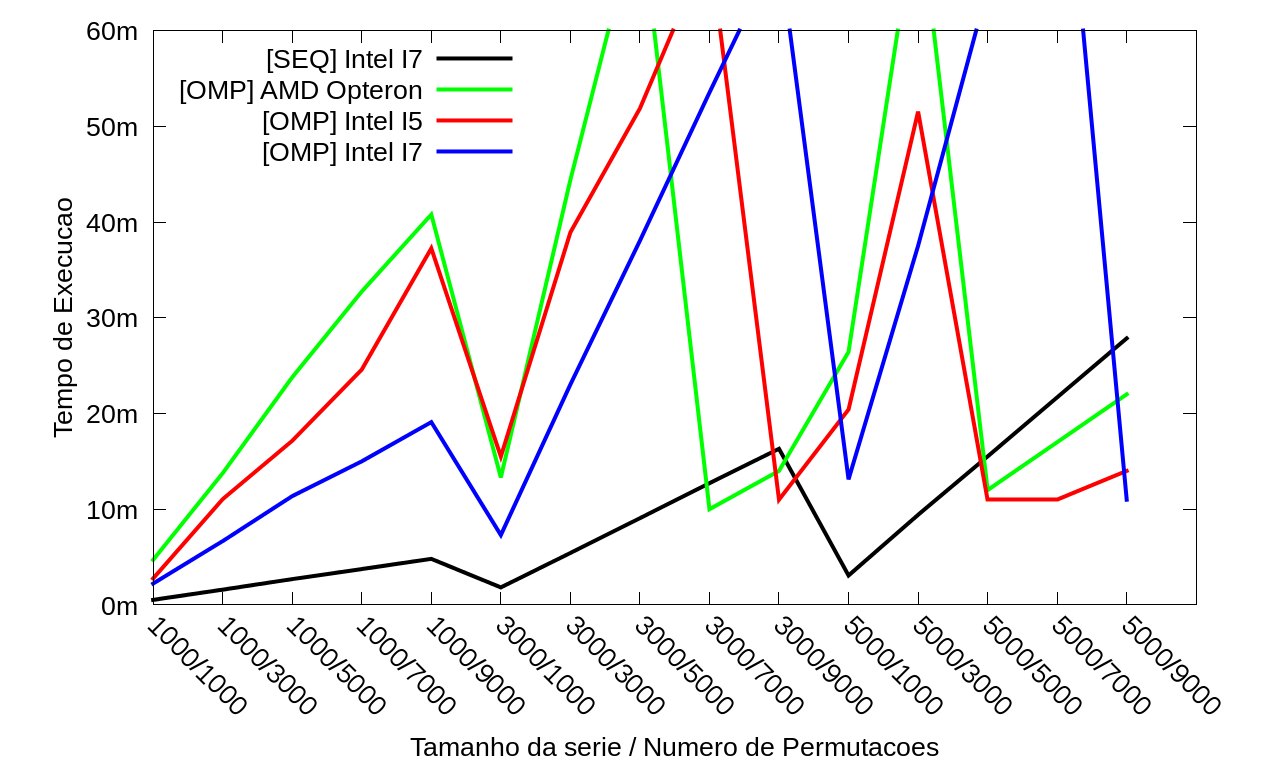
\includegraphics[width=1.0\textwidth]{Imagens/graficos_mcarlo/mcarlo_tempos_omp.png}
\caption{Gráfico de tempo do algoritmo Monte Carlo}
\label{fig:grafico_tempo_mcarlo_omp}
\end{figure}
%%%%%%%%%%%%%%%%%%%%%%%%%%%%%%%%%%%%%%%%%%%%%%%%%%%%%%%%%%

%%%%%%%%%%%%%%%%%%%%%%%%%%%%%%%%%%%%%%%%%%%%%%%%%%%%%%%%%%
% FIGURA
\begin{figure}[H]
\centering
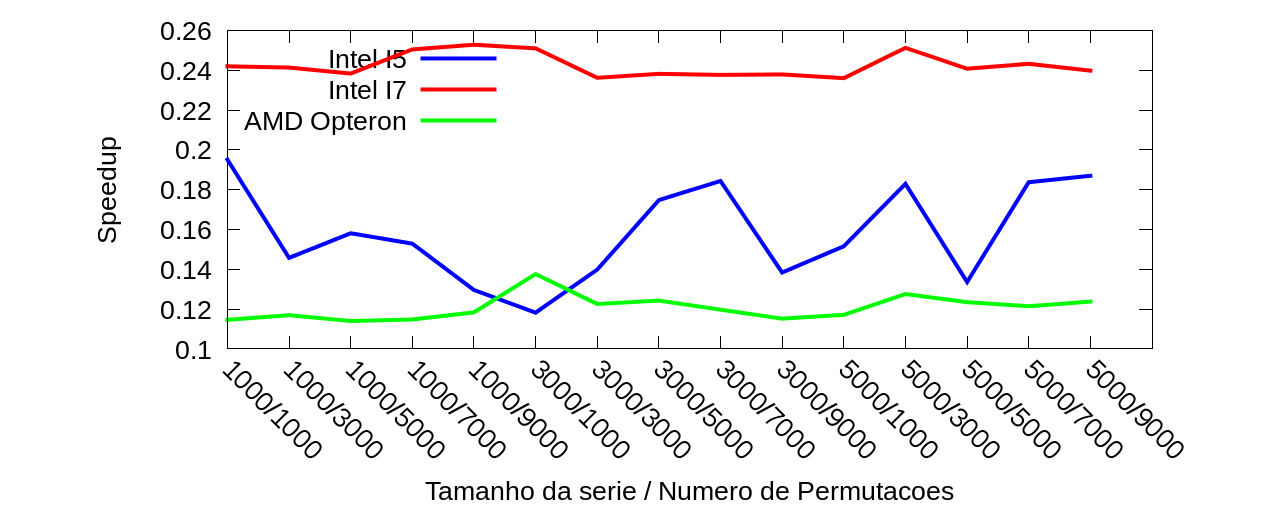
\includegraphics[width=1.0\textwidth]{Imagens/graficos_mcarlo/mcarlo_speedup_omp.png}
\caption{Gráfico do speedup do algoritmo Monte Carlo}
\label{fig:grafico_speedup_mcarlo_omp}
\end{figure}
%%%%%%%%%%%%%%%%%%%%%%%%%%%%%%%%%%%%%%%%%%%%%%%%%%%%%%%%%%

%%%%%%%%%%%%%%%%%%%%%%%%%%%%%%%%%%%%%%%%%%%%%%%%%%%%%%%%%%
% FIGURA
\begin{figure}[H]
\centering
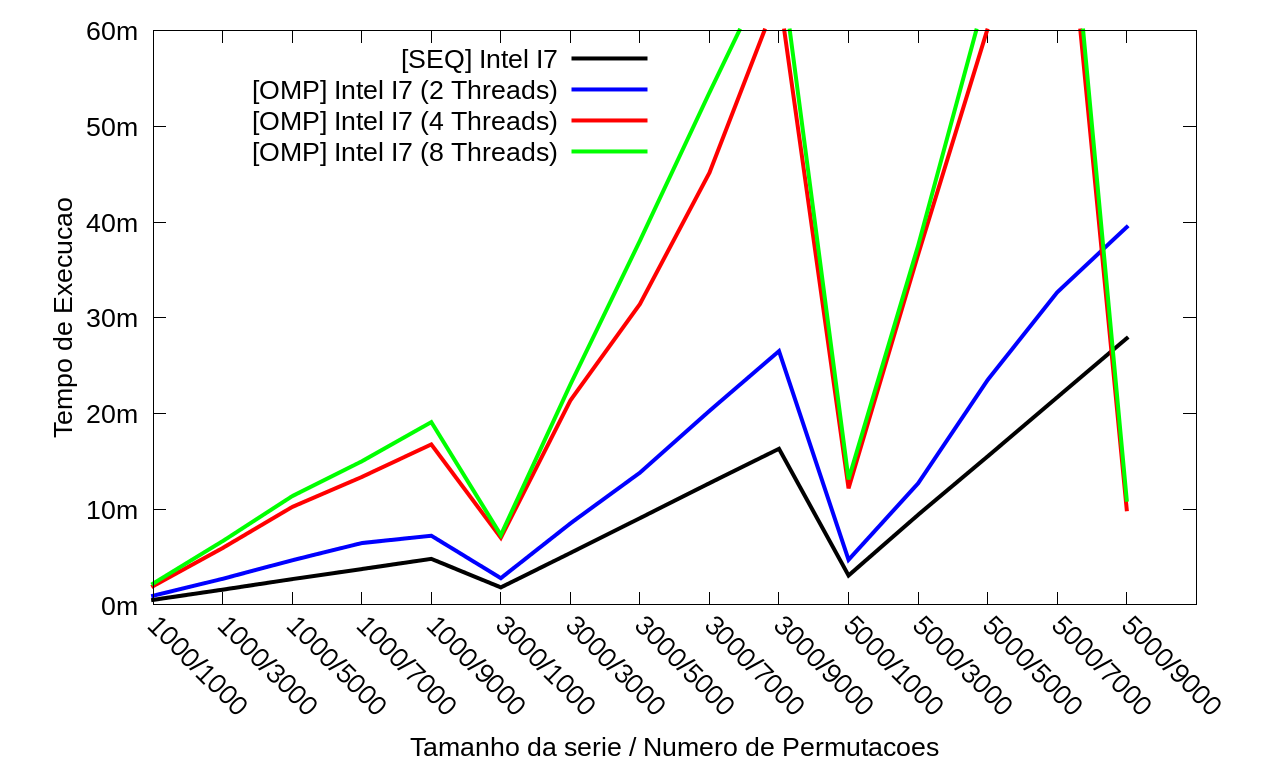
\includegraphics[width=1.0\textwidth]{Imagens/graficos_mcarlo/mcarlo_tempos_omp_threads.png}
\caption{Gráfico de tempo do algoritmo Monte Carlo}
\label{fig:grafico_speedup_mcarlo_omp_threads}
\end{figure}
%%%%%%%%%%%%%%%%%%%%%%%%%%%%%%%%%%%%%%%%%%%%%%%%%%%%%%%%%%

%%%%%%%%%%%%%%%%%%%%%%%%%%%%%%%%%%%%%%%%%%%%%%%%%%%%%%%%%%
% FIGURA
\begin{figure}[H]
\centering
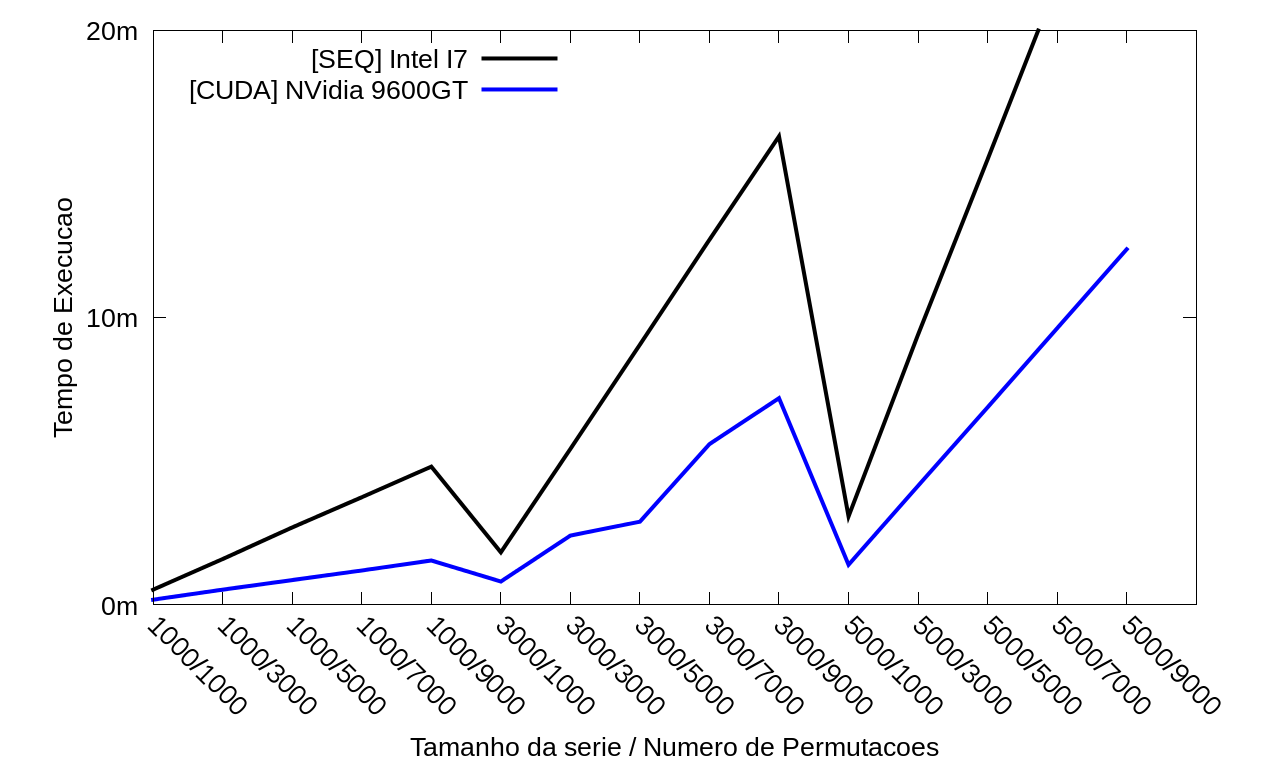
\includegraphics[width=1.0\textwidth]{Imagens/graficos_mcarlo/mcarlo_tempos_cuda.png}
\caption{Gráfico de tempo do algoritmo Monte Carlo}
\label{fig:grafico_tempo_mcarlo_cuda}
\end{figure}
%%%%%%%%%%%%%%%%%%%%%%%%%%%%%%%%%%%%%%%%%%%%%%%%%%%%%%%%%%

%%%%%%%%%%%%%%%%%%%%%%%%%%%%%%%%%%%%%%%%%%%%%%%%%%%%%%%%%%
% FIGURA
\begin{figure}[H]
\centering
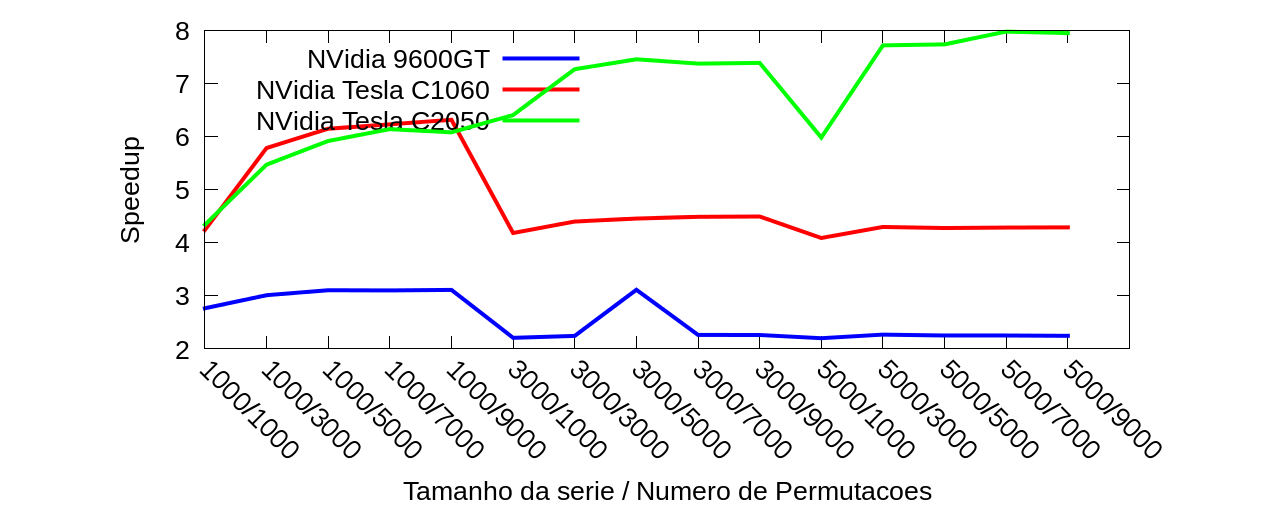
\includegraphics[width=1.0\textwidth]{Imagens/graficos_mcarlo/mcarlo_speedup_cuda.png}
\caption{Gráfico do speedup do algoritmo Monte Carlo}
\label{fig:grafico_speedup_mcarlo_cuda}
\end{figure}
%%%%%%%%%%%%%%%%%%%%%%%%%%%%%%%%%%%%%%%%%%%%%%%%%%%%%%%%%%

\section{Análise dos resultados}

Como podemos ver, mesmo sem nenhuma otimização tanto no código quanto nos parâmetros de execução do Kernel, os tempos de execução da versão CUDA são significantemente menores, apresentando tempos 6 vezes menores quando usado a GPU 9600GT, e de até 40 vezes com a GPU GTX480 nos testes feitos. Além disso, é perceptível pelas curvas apresentadas no gráfico que essa redução será ainda maior a medida que o tamanho da entrada aumentar, comprovando o poder de processamento das GPUs Nvidia com a tecnologia CUDA.